\documentclass[pra,twocolumn,superscriptaddress,longbibliography,floatfix]{revtex4-2}

\usepackage{amsmath,amssymb,bm}
\usepackage{graphicx}
\usepackage{booktabs}
\usepackage{multirow}
\usepackage{xcolor}
\usepackage[colorlinks=true,linkcolor=blue!55!black,citecolor=blue!55!black,urlcolor=blue!55!black]{hyperref}

\newcommand{\Tr}{\operatorname{Tr}}
\newcommand{\ket}[1]{\left|#1\right\rangle}
\newcommand{\bra}[1]{\left\langle#1\right|}
\newcommand{\braket}[2]{\left\langle#1\middle|#2\right\rangle}
\newcommand{\ketbra}[2]{\left|#1\right\rangle\!\left\langle#2\right|}
\newcommand{\dd}{\mathrm{d}}
\newcommand{\Erel}{E_{\rm rel}}
\newcommand{\Scl}{S_{\rm cl}}
\newcommand{\SW}{S_{W}}
\newcommand{\epsp}{\varepsilon_{+}}
\newcommand{\epsm}{\varepsilon_{-}}

\begin{document}

\title{Classical versus quantum entanglement entropy of coupled rotors:\\
a universal deficit $1-\ln2$ and its phase-space origin}

\author{[Author list to be completed]}
\affiliation{[Affiliation]}

\date{\today}

\begin{abstract}
We compare the entanglement entropy of eigenstates of two rotors coupled by
$\lambda\cos(\theta_{1}-\theta_{2})$ --- the phase model of two
Josephson-coupled condensates, or two stacked planar dipolar rotors --- with
the Boltzmann entropy of the reduced classical microcanonical distribution and
with the entropies of the Wigner and Husimi distributions. Conservation of total
angular momentum makes the reduced density matrix diagonal and fixes the
phase-space cell at $h$, so the comparison contains no adjustable constant.
Every sector is an exact Mathieu problem. At weak coupling the $O(\lambda^{2})$
normalization of the perturbed state supplies the entire linear entropy. Deep in
the rotation regime the Schmidt weights are $J_{j}^{2}(\gamma)$, the classical
weights follow the arcsine law, and the quantum entropy lies below the classical
one by the universal constant $1-\ln2$, approached as $\gamma^{-1/3}$. Both
entropies peak near the separatrix. The Wigner function of the reduced state
reproduces the von Neumann entropy identically; the constant $1-\ln2$ is the
entropy carried by the chord (interference) terms of the two-rotor Wigner
function. The Husimi (Wehrl) entropy exceeds the von Neumann entropy by
$(1-\ln2)-D(\sigma)$ with $D(\sigma)\simeq0.080/\sigma$ for coherent-state
width $\sigma$: smoothing restores the classical value only as $\sigma\to\infty$,
and the width takes over the role of the arbitrary phase-space cell of the
coupled-oscillator problem.
\end{abstract}

\maketitle

%=============================================================================
\section{Introduction}
\label{sec:intro}
%=============================================================================

How much of the entanglement of a highly excited eigenstate can be obtained from
a purely classical calculation? Duan, Kovner and Skokov (DKS)~\cite{DKS} posed
this question for two coupled harmonic oscillators,
\begin{equation}
H_{c}=\tfrac12\left(p_{x}^{2}+p_{y}^{2}+\omega^{2}x^{2}+\Omega^{2}y^{2}
+2Cxy\right),
\label{eq:DKS}
\end{equation}
with $C\ll\omega^{2}\ll\Omega^{2}$. They integrated the microcanonical
distribution over the second oscillator, computed the Boltzmann entropy of the
reduced distribution, and found it equal to the von Neumann entropy of the
reduced density matrix of a WKB eigenstate,
$S=\ln[\pi C\sqrt{E_{1}E_{2}}/(\hbar\omega\Omega^{2})]$, provided the
phase-space cell is taken to be $h/2$. Any other cell shifts the classical
entropy by a constant. The question is motivated by high-energy scattering, where
the entanglement of the probed degrees of freedom has been argued to appear as
the Boltzmann entropy of the final state~\cite{KharzeevLevin,Kutak,Hagiwara}.

The oscillator pair is Gaussian, its phase space is non-compact (so the cell is
not fixed by the theory), and it has no separatrix. Two rotors on a circle,
\begin{equation}
H=\frac{p_{1}^{2}}{2I}+\frac{p_{2}^{2}}{2I}
+\lambda\cos\left(\theta_{1}-\theta_{2}\right),
\label{eq:H}
\end{equation}
remove all three restrictions while remaining solvable. The model is realized in
several settings. For two Bose--Einstein condensates coupled by tunneling, or two
superconducting islands coupled by a Josephson junction, $\theta_{i}$ is the
phase and $m_{i}=p_{i}/\hbar$ the particle number of mode $i$; in the Josephson
regime, where the number imbalance is small compared with the total number,
the two-mode Hamiltonian reduces to Eq.~\eqref{eq:H} with
$\hbar^{2}/I$ the charging (interaction) energy and $\lambda$ the Josephson
energy~\cite{Smerzi97,Raghavan99,GatiOberthaler,FazioReview}. The separatrix of
the relative motion is then the boundary between Josephson oscillations and
running-phase (self-trapped) motion~\cite{Smerzi97,Raghavan99,Albiez05}, and the
entanglement between the two rotors is the mode entanglement of the two
condensates~\cite{Hines03}. Two planar rotors carrying dipoles $d$, rotating in
parallel planes a distance $R$ apart along their common axis, interact through
exactly $\lambda\cos(\theta_{1}-\theta_{2})$ with $\lambda=d^{2}/4\pi\epsilon_{0}R^{3}$,
because the dipoles are perpendicular to the separation.

We carry out the DKS comparison for Eq.~\eqref{eq:H} and extend it to the
Wigner and Husimi distributions, whose information-theoretic content is of
independent interest~\cite{Wehrl,PSinfo1,PSinfo2}. Our main results are as
follows.

(i) Conservation of total angular momentum fixes the Schmidt basis and the
phase-space cell, and every sector is an exact Mathieu problem
(Sec.~\ref{sec:model}).

(ii) At weak coupling the entropy is controlled by the $O(\lambda^{2})$
normalization of the perturbed state, which supplies the whole linear entropy
(Sec.~\ref{sec:weak}).

(iii) Deep in rotation the Schmidt weights are squared Bessel functions and the
classical weights follow the arcsine law; the quantum entropy lies below the
classical one by $1-\ln2$ (Sec.~\ref{sec:rotation}). At generic energies the
deficit grows towards the same constant, and both entropies are maximal near the
separatrix (Sec.~\ref{sec:compare}). In deep libration we obtain the entropy
including the first anharmonic correction (Sec.~\ref{sec:libration}).

(iv) The reduced Wigner function returns the von Neumann entropy identically,
and $1-\ln2$ is the entropy of the chord terms of the Wigner function. The
Wehrl entropy recovers a fraction $1-D(\sigma)/(1-\ln2)$ of the deficit, with
$D$ in closed form (Sec.~\ref{sec:wigner}).

Derivations are collected in the appendixes, and every analytic statement has
been checked numerically (Appendix~\ref{app:num}).

%=============================================================================
\section{Model and exact reduction}
\label{sec:model}
%=============================================================================

\subsection{Conservation laws and relative motion}

In the basis $\braket{\theta_{1},\theta_{2}}{m_{1},m_{2}}=
e^{im_{1}\theta_{1}+im_{2}\theta_{2}}/2\pi$, $m_{i}\in\mathbb{Z}$, the free
energies are $\hbar^{2}(m_{1}^{2}+m_{2}^{2})/2I$ and the coupling has matrix
elements
\begin{equation}
\bra{m_{1}',m_{2}'}\cos(\theta_{1}-\theta_{2})\ket{m_{1},m_{2}}
=\tfrac12\,\delta_{m_{1}',m_{1}\pm1}\,\delta_{m_{2}',m_{2}\mp1},
\label{eq:V}
\end{equation}
transferring one quantum of angular momentum between the rotors. The total
angular momentum $J=p_{1}+p_{2}=\hbar M$ is conserved. Within a sector we use
\begin{equation}
k=\frac{m_{1}-m_{2}}{2},\qquad n=2k,\qquad
m_{1,2}=\frac{M}{2}\pm k,
\label{eq:k}
\end{equation}
with $k\in\mathbb{Z}$ for even $M$ and $k\in\mathbb{Z}+\tfrac12$ for odd $M$, and
the dimensionless coupling $\alpha=\lambda I/2\hbar^{2}$.

Classically, the canonical variables $\Theta=(\theta_{1}+\theta_{2})/2$,
$\varphi=\theta_{1}-\theta_{2}$, $J$, and $p=(p_{1}-p_{2})/2$ give
\begin{equation}
H=\frac{J^{2}}{4I}+H_{\rm rel},\qquad
H_{\rm rel}=\frac{p^{2}}{I}+\lambda\cos\varphi .
\label{eq:Hcm}
\end{equation}
The relative motion is a pendulum with moment of inertia $\mu=I/2$, potential
minimum at $\varphi=\pi$, and separatrix at $\Erel\equiv E-J^{2}/4I=\lambda$; for
$|\Erel|<\lambda$ the relative angle librates, for $\Erel>\lambda$ it circulates.
Quantum mechanically $p=\hbar k$.

\subsection{Each sector is a Mathieu problem}

With $m_{1}^{2}+m_{2}^{2}=M^{2}/2+2k^{2}$, the Hamiltonian restricted to sector
$M$ is $\hbar^{2}M^{2}/4I+h$ with
\begin{equation}
h_{kk'}=\frac{\hbar^{2}}{I}k^{2}\,\delta_{kk'}
+\frac{\lambda}{2}\left(\delta_{k',k+1}+\delta_{k',k-1}\right).
\label{eq:hsector}
\end{equation}
Writing $\Psi=e^{iM\Theta}u(\varphi)/\sqrt{2\pi}$ with
$u=\sum_{k}c_{k}e^{ik\varphi}/\sqrt{2\pi}$, Eq.~\eqref{eq:hsector} is the matrix
of $h=-(\hbar^{2}/I)\,\dd^{2}/\dd\varphi^{2}+\lambda\cos\varphi$ in the plane-wave
basis: each sector is exactly the quantum pendulum $H_{\rm rel}$, with periodic
($M$ even) or antiperiodic ($M$ odd) boundary conditions. With $\varphi=2z$,
\begin{equation}
\begin{gathered}
u''+(a-2q\cos2z)u=0,\\
a=\frac{4I\Erel}{\hbar^{2}},\qquad q=\frac{2\lambda I}{\hbar^{2}}=4\alpha,
\end{gathered}
\label{eq:mathieu}
\end{equation}
the Mathieu equation~\cite{DLMF28}. The relative energies are
$\hbar^{2}/4I$ times $a_{0}<b_{2}<a_{2}<\dots$ ($M$ even) or
$b_{1}<a_{1}<b_{3}<\dots$ ($M$ odd), the separatrix is at $a=2q$, and the
Bohr--Sommerfeld area inside the separatrix, $8\sqrt{2I\lambda}$, gives
$N_{\rm lib}\simeq(4/\pi)\sqrt{q}$ librating levels ($25.5$ and $50.9$ for
$\lambda I/\hbar^{2}=200$ and $800$, against $25$ and $51$ counted).

\subsection{The entanglement entropy is a Shannon entropy}
\label{sec:S}

An eigenstate in sector $M$ is
$\ket\Psi=\sum_{k}c_{k}\ket{\tfrac M2+k,\tfrac M2-k}$. Distinct $k$ carry
distinct rotor-2 labels, so the partial trace removes every cross term:
\begin{equation}
\begin{gathered}
\rho_{1}=\sum_{k}p_{k}\ketbra{\tfrac M2+k}{\tfrac M2+k},\qquad p_{k}=|c_{k}|^{2},\\
S_{q}=-\sum_{k}p_{k}\ln p_{k},
\end{gathered}
\label{eq:Smathieu}
\end{equation}
exactly. The entanglement entropy is the Shannon entropy of the Fourier
coefficients of a Mathieu function, and the Schmidt basis is the
angular-momentum basis at every energy and coupling. This is the structural fact
on which everything below rests.

\subsection{Exchange symmetry and branch states}
\label{sec:ln2}

The exchange $\theta_{1}\leftrightarrow\theta_{2}$ maps $k\to-k$, so exact
eigenstates have $c_{-k}=\pm c_{k}$. Above the separatrix the levels form
doublets whose members are the even and odd combinations of two branch states
$\ket{\Psi_{\pm n}}$, describing relative rotation in the two senses; the
splitting vanishes as $\lambda^{|n|}$ at weak coupling and exponentially in the
semiclassical regime. If the branch weights $q_{k}$ are supported on $k>0$, the
parity eigenstate has $p_{\pm k}=q_{k}/2$ and
\begin{equation}
S_{\rm exact}=\ln2+S_{\rm branch}.
\label{eq:Sln2}
\end{equation}
Since $\rho_{1}$ is diagonal, no cross term can contribute; only overlapping
supports could. Classically the two branches are the two invariant tori
$p\gtrless0$, which the microcanonical distribution weights equally, so the same
$\ln2$ appears on both sides. Numerically we diagonalize Eq.~\eqref{eq:hsector}
separately in the two parity sectors (Appendix~\ref{app:num}).

%=============================================================================
\section{Weak coupling and the normalization term}
\label{sec:weak}
%=============================================================================

Expand about $\ket{0}\equiv\ket{m_{1},m_{2}}$ with $n=m_{1}-m_{2}\notin
\{\pm1,\pm2\}$ (at $n=\pm1,\pm2$ the exchange partner is reached at first or
second order). Rayleigh--Schr\"odinger theory in intermediate normalization
(Appendix~\ref{app:pt}) gives $E^{(1)}=0$,
\begin{equation}
E^{(2)}=\frac{\lambda^{2}I}{2\hbar^{2}\left(n^{2}-1\right)},
\label{eq:E2}
\end{equation}
first-order amplitudes $c_{\pm}=\mp\alpha/(n\pm1)$ on $\ket{m_{1}\pm1,m_{2}\mp1}$
and second-order amplitudes $c_{\pm\pm}=\alpha^{2}/[2(n\pm1)(n\pm2)]$ on
$\ket{m_{1}\pm2,m_{2}\mp2}$. The normalization factor is
$\mathcal{N}=1-\tfrac12(\epsp+\epsm)+O(\lambda^{4})$ with
\begin{equation}
\varepsilon_{\pm}=c_{\pm}^{2}=\frac{\alpha^{2}}{(n\pm1)^{2}} .
\label{eq:eps}
\end{equation}
In the state, $\mathcal{N}-1$ is of the order to which the state is not kept and
is routinely dropped. In the density matrix it cannot be: $\rho$ is bilinear in
the amplitudes, so the $\ketbra00$ element is $\mathcal{N}^{2}=1-\epsp-\epsm$, an
$O(\lambda^{2})$ correction of the same order as the populations
$\varepsilon_{\pm}$. By Eq.~\eqref{eq:Smathieu} all coherences drop out of the
partial trace (including the second-order amplitudes, which pair with $\ket0$
through different rotor-2 labels), and
\begin{equation}
\begin{split}
\rho_{1}={}&\left(1-\epsp-\epsm\right)\ketbra{m_{1}}{m_{1}}\\
&+\epsp\ketbra{m_{1}{+}1}{m_{1}{+}1}+\epsm\ketbra{m_{1}{-}1}{m_{1}{-}1},
\end{split}
\label{eq:rho1}
\end{equation}
with error $O(\lambda^{4})$. Hence
\begin{align}
S&=\epsp\ln\frac{1}{\epsp}+\epsm\ln\frac{1}{\epsm}+\left(\epsp+\epsm\right)
+O(\varepsilon^{2}),\label{eq:Sweak}\\
S_{L}&=1-\Tr\rho_{1}^{2}=2\left(\epsp+\epsm\right)+O(\varepsilon^{2}).
\label{eq:SL}
\end{align}
The non-logarithmic term of $S$ and the whole of $S_{L}$ come from the
normalization: with $p_{0}=1$ one would find $\Tr\rho_{1}=1+\epsp+\epsm$ and
$S_{L}<0$, and the von Neumann entropy would be low by a relative amount
$1/[1+\ln(1/\varepsilon)]$, which vanishes only logarithmically as
$\lambda\to0$ ($10$--$14\%$ for $\lambda I/\hbar^{2}=0.02$--$0.2$ at $n=0$,
Fig.~\ref{fig:weak}). The same structure appears in the oscillator ground state
of Ref.~\cite{DKS}, $S=-(1-f)\ln(1-f)-f\ln f$ with $f=C^{2}/4\omega\Omega^{3}$,
where $-(1-f)\ln(1-f)$ is the normalization contribution. For $|n|\ge3$ the
exact parity eigenstates have entropy $\ln2$ plus Eq.~\eqref{eq:Sweak}, by
Eq.~\eqref{eq:Sln2}, since the two branches overlap only at
$O(\lambda^{|n|})$.

For $|n|\gg1$, $\epsp\simeq\epsm\simeq\gamma^{2}/4$ with
\begin{equation}
\gamma\equiv\frac{\lambda I}{\hbar^{2}n}=\frac{2\alpha}{n},\qquad
S\simeq\gamma^{2}\left[\ln\frac{2}{\gamma}+\frac12\right].
\label{eq:Sasym}
\end{equation}
The factor $2$ in the logarithm is easily lost; with it, Eq.~\eqref{eq:Sasym}
agrees with Eq.~\eqref{eq:Sweak} to $0.3\%$ at $n=30$. We shall recover
Eq.~\eqref{eq:Sasym} as the small-$\gamma$ limit of an exact solution.

\begin{figure*}[t]
\centering
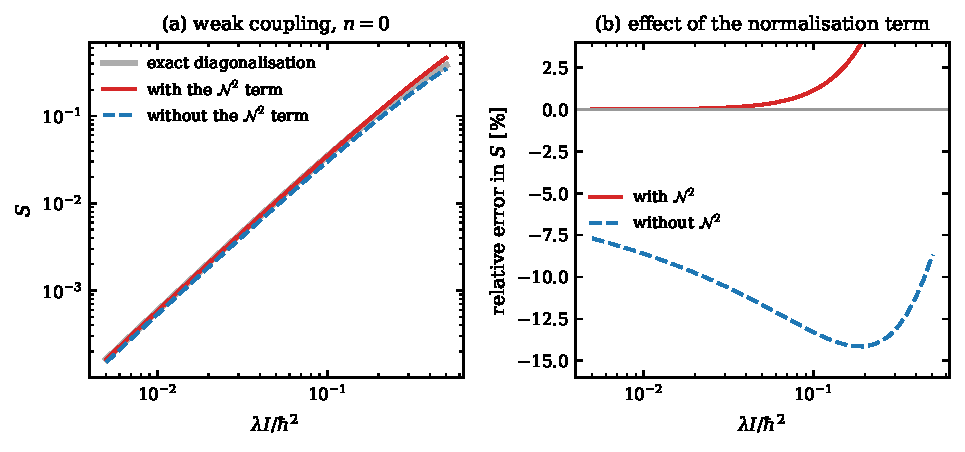
\includegraphics[width=0.85\textwidth]{fig1_weak.pdf}
\caption{Weak coupling, $n=0$ ($m_{1}=m_{2}=4$). (a) Entanglement entropy from
exact diagonalization (grey), Eq.~\eqref{eq:Sweak} (red), and the same expression
with the normalization term removed (blue dashed). (b) Relative error of the two
truncations: with the term, $0.05\%$ at $\lambda I/\hbar^{2}=0.02$ and $1\%$ at
$0.1$, decreasing as $\lambda^{2}$; without it, $10$--$14\%$, not vanishing as
$\lambda\to0$.}
\label{fig:weak}
\end{figure*}

%=============================================================================
\section{The classical reduced distribution}
\label{sec:classical}
%=============================================================================

Following Ref.~\cite{DKS}, the classical counterpart of an eigenstate with
energy $E$ and total angular momentum $J$ is the microcanonical distribution
\begin{equation}
W_{\rm cl}=\mathcal{C}\,\delta(E-H)\,\delta(J-p_{1}-p_{2}).
\label{eq:Wjoint}
\end{equation}
Integrating over $(\theta_{2},p_{2})$, the second delta function sets
$p_{2}=J-p_{1}$, and the first has two roots $\varphi=\pm\arccos\xi$,
$\xi=(\Erel-p^{2}/I)/\lambda$, with $p=p_{1}-J/2$. The reduced distribution is
\begin{equation}
W_{\rm cl}(\theta_{1},p_{1})=\frac{2\mathcal{C}\;
\Theta\big(\lambda-|\Erel-p^{2}/I|\big)}
{\sqrt{\lambda^{2}-\left(\Erel-p^{2}/I\right)^{2}}},
\label{eq:Wclass}
\end{equation}
independent of $\theta_{1}$. The two roots $\pm\arccos\xi$ --- two relative angles
compatible with one momentum of rotor 1 --- are the two branches whose quantum
interference is the subject of Secs.~\ref{sec:rotation} and \ref{sec:wigner}.

The support is $|p|\le\sqrt{I(\Erel+\lambda)}$ in libration and
$\sqrt{I(\Erel-\lambda)}\le|p|\le\sqrt{I(\Erel+\lambda)}$ in rotation. Its length
$L(\Erel)$ grows through libration, peaks at $2\sqrt{2I\lambda}$ at the
separatrix, and falls above it with infinite slope: a cusp maximum, which bounds
the entropy by $\ln(L/\hbar)$. The momentum density $w=2\pi W_{\rm cl}$ is
normalized by $\mathcal{C}=1/8\pi B$, with the band integral
(Appendix~\ref{app:integrals})
\begin{equation}
B=\begin{cases}
\sqrt{\dfrac{I}{\Erel+\lambda}}\,\mathsf{K}\!\left(\sqrt{\dfrac{2\lambda}{\Erel+\lambda}}\right),
& \Erel>\lambda,\\[12pt]
\sqrt{\dfrac{I}{2\lambda}}\,\mathsf{K}\!\left(\sqrt{\dfrac{\Erel+\lambda}{2\lambda}}\right),
& |\Erel|<\lambda,
\end{cases}
\label{eq:B}
\end{equation}
where $\mathsf{K}$ is the complete elliptic integral of the first kind; $2B$ is
the period of the relative motion, so $w\,\dd p_{1}$ is the fraction of the
period spent in $\dd p_{1}$.

\emph{The cell.} The Boltzmann entropy
$-\int W_{\rm cl}\ln(W_{\rm cl}\Delta)$ requires a cell $\Delta$. On a compact
configuration space it is fixed: $p_{1}=\hbar m_{1}$, and each quantum state
occupies the strip $2\pi\times\hbar=h$. With $\Delta=h$,
$\Scl=-\int\dd p_{1}\,w\ln(w\hbar)$. The quantity with the same status as
Eq.~\eqref{eq:Smathieu} is the Shannon entropy $\Scl^{\rm bin}$ of the cell
weights $w_{m}=\int_{\hbar(m-1/2)}^{\hbar(m+1/2)}w\,\dd p_{1}$. One has
$\Scl^{\rm bin}\ge\Scl$, the difference being a sum of relative entropies
concentrated in the cells that contain the band-edge singularities. Neither
comparison contains an adjustable constant.

%=============================================================================
\section{Deep rotation and the constant $1-\ln2$}
\label{sec:rotation}
%=============================================================================

\subsection{Wannier--Stark ladder and Bessel weights}

For $k=n/2+j$ with $n\gg1$, $\hbar^{2}k^{2}/I=\hbar^{2}n^{2}/4I+Fj+\hbar^{2}j^{2}/I$
with $F=\hbar^{2}n/I$. Dropping the quadratic term, which is smaller than the
linear one by $|j|/n$, turns Eq.~\eqref{eq:hsector} into the Wannier--Stark
problem $Fjc_{j}+\tfrac{\lambda}{2}(c_{j+1}+c_{j-1})=Ec_{j}$~\cite{Wannier,Fukuyama}.
The Bessel recurrence $J_{\nu-1}+J_{\nu+1}=(2\nu/x)J_{\nu}$ shows that
$c_{j}=J_{j-s}(-\lambda/F)$ is an eigenvector with eigenvalue $Fs$, so
\begin{equation}
p_{j}=J_{j-s}^{2}(\gamma),\qquad \gamma=\frac{\lambda}{F}=\frac{\lambda I}{\hbar^{2}n},
\label{eq:bessel}
\end{equation}
valid for $\gamma/n=\lambda/4\Erel\ll1$. Exact diagonalization confirms
Eq.~\eqref{eq:bessel} pointwise to $3\times10^{-3}$ at $\gamma/n=0.01$, and the
entropy to four or five digits for $n=100$--$400$. The Bessel eigenvector is a
branch state, and its entropy
\begin{equation}
S_{\rm branch}(\gamma)=-\sum_{j}J_{j}^{2}(\gamma)\ln J_{j}^{2}(\gamma)
\label{eq:SB}
\end{equation}
is a universal function of $\gamma$ (Fig.~\ref{fig:rotation}). For small $\gamma$,
$J_{0}^{2}\simeq1-\gamma^{2}/2$ and $J_{\pm1}^{2}\simeq\gamma^{2}/4$ reproduce
Eq.~\eqref{eq:Sasym}, the depletion of $J_{0}^{2}$ being the normalization term
of Sec.~\ref{sec:weak}.

In the same limit the classical density~\eqref{eq:Wclass}, linearized about
$p_{0}=\hbar n/2$, becomes the arcsine law of half-width $\gamma$,
\begin{equation}
w(j)=\frac{1}{\pi\sqrt{\gamma^{2}-j^{2}}},\qquad
\Scl^{\rm branch}=\ln\frac{\pi\gamma}{2},
\label{eq:arcsine}
\end{equation}
so that for the two bands of a parity eigenstate
$\Scl=\ln(\pi\gamma)=\ln[(\pi\lambda/2\hbar)\sqrt{I/\Erel}]$, the rotor
counterpart of the DKS result.

\subsection{Fringes and the entropy deficit}

The Debye expansion of $J_{j}(\gamma)$ with $j=\gamma\cos\beta$~\cite{DLMF10}
gives
\begin{equation}
\begin{gathered}
J_{j}^{2}(\gamma)\simeq w(j)\left[1+\cos\Phi_{j}\right],\\
\Phi_{j}=2\sqrt{\gamma^{2}-j^{2}}-2j\arccos\frac{j}{\gamma}-\frac{\pi}{2},
\end{gathered}
\label{eq:fringes}
\end{equation}
fringes of \emph{full} contrast about the classical weights, with local
wavenumber $\dd\Phi_{j}/\dd j=-2\beta\in(-2\pi,0)$. The same holds at any energy:
the WKB ansatz $c_{k}=A_{k}e^{i\chi_{k}}$ for the difference equation
$\hbar^{2}k^{2}c_{k}/I+\tfrac{\lambda}{2}(c_{k+1}+c_{k-1})=\Erel c_{k}$ gives a
local wavenumber $\phi_{k}$ with $\Erel-\hbar^{2}k^{2}/I=\lambda\cos\phi_{k}$ ---
the classical relative angle --- and constancy of the Casoratian gives
$|A_{k}|^{2}\propto[\lambda^{2}-(\Erel-\hbar^{2}k^{2}/I)^{2}]^{-1/2}$, the
classical density. A real eigenvector superposes the two waves $\pm\phi_{k}$, so
\begin{equation}
p_{k}\simeq w_{k}\left(1+\cos\Phi_{k}\right),\qquad
\Phi_{k+1}-\Phi_{k}=2\phi_{k}.
\label{eq:fringesgen}
\end{equation}
Inserting this into Eq.~\eqref{eq:Smathieu}, the cross term
$\sum w_{k}\cos\Phi_{k}\ln w_{k}$ averages out and the phases are equidistributed
wherever $2\phi_{k}\not\approx0\bmod2\pi$, so
\begin{equation}
\Scl-S_{q}\;\to\;\frac{1}{2\pi}\int_{0}^{2\pi}
(1+\cos\Phi)\ln(1+\cos\Phi)\,\dd\Phi=1-\ln2
\label{eq:main}
\end{equation}
(Appendix~\ref{app:integrals}). The limiting deficit $1-\ln2=0.30685$ is
universal: it depends only on the full contrast of the two-branch interference.
Equidistribution fails near the band edges (caustics), where the fringes become
stationary; the phase accumulated over the last $\delta$ cells,
$\simeq\tfrac{4\sqrt2}{3}\delta^{3/2}/\sqrt\gamma$, reaches $2\pi$ at
$\delta\sim\gamma^{1/3}$, whose arcsine weight is $\sim\gamma^{-1/3}$. Hence
$\Scl-S_{q}=1-\ln2-O(\gamma^{-1/3})$. Summing the Bessel weights directly,
$\Scl^{\rm bin}-S_{q}=0.233$, $0.270$, $0.288$ and $0.298$ at
$\gamma=10^{3},10^{4},10^{5},10^{6}$, the distance to $1-\ln2$ falling by close
to $10^{1/3}$ per decade [Fig.~\ref{fig:rotation}(b)].

\begin{figure*}[t]
\centering
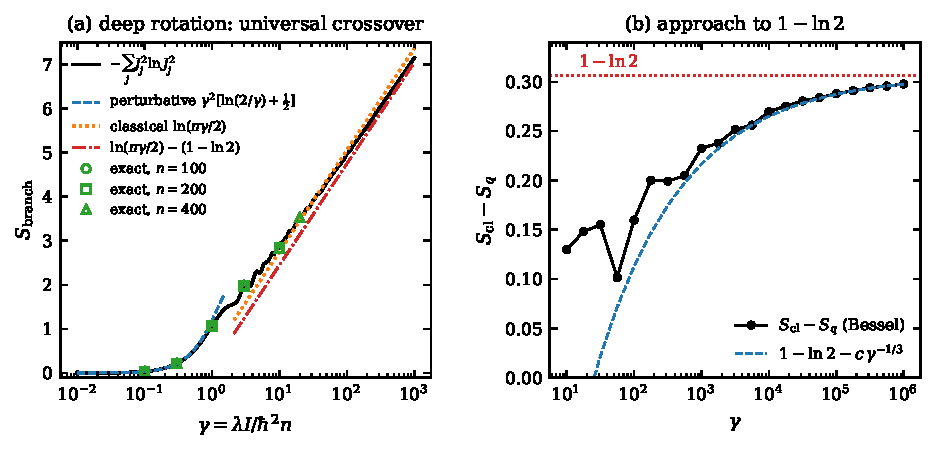
\includegraphics[width=0.92\textwidth]{fig2_rotation.pdf}
\caption{Deep rotation. (a) Branch entropy as a function of
$\gamma=\lambda I/\hbar^{2}n$: Bessel result~\eqref{eq:SB} (black), its
small-$\gamma$ limit~\eqref{eq:Sasym} (blue dashed), classical arcsine entropy
(orange dotted), and classical entropy minus $1-\ln2$ (red dash-dotted). Open
symbols: exact diagonalization at $n=100,200,400$. (b) Deficit
$\Scl^{\rm bin}-S_{q}$ from the Bessel weights, approaching $1-\ln2$ as
$\gamma^{-1/3}$.}
\label{fig:rotation}
\end{figure*}

\emph{Why oscillators and rotors differ.} For the oscillators no conservation law
selects a Schmidt basis; the reduced density matrix of Ref.~\cite{DKS} is doubly
degenerate with smooth arcsine eigenvalues, and the two-branch interference is
absorbed into the eigenvectors. For the rotors, conservation of $J$ fixes the
Schmidt basis (Sec.~\ref{sec:S}), so the interference appears in the eigenvalues
as the fringes~\eqref{eq:fringesgen}. The leading logarithms agree; the
constants differ by $1-\ln2$. Equivalently, the classical formula reproduces the
quantum entropy if the cell is taken to be $eh/2$ instead of $h$.

%=============================================================================
\section{Generic energies and the separatrix}
\label{sec:compare}
%=============================================================================

Figure~\ref{fig:separatrix} compares $S_{q}$ from exact diagonalization with
$\Scl^{\rm bin}$ from quadrature of Eq.~\eqref{eq:Wclass} for
$\lambda I/\hbar^{2}=50$, $200$ and $800$. The curves track each other over the
whole spectrum. In libration the quantum entropy lies below the classical one by
about $0.2$ (except near the bottom of the well, where the band covers only a
few cells); in rotation by a smaller amount that grows with $\lambda$.
Figure~\ref{fig:fringes}(a) shows the mechanism at $\lambda I/\hbar^{2}=800$,
$\Erel/\lambda=1.54$: the quantum weights oscillate about the classical envelope
with full contrast, and although the total-variation distance between the two
distributions is $0.33$, the entropies differ by less than $1\%$. Averaged over
$0.2\le\Erel/\lambda\le0.7$ and $1.5\le\Erel/\lambda\le2.5$, the deficit grows
from $0.18$ to $0.24$ (libration) and from $0.01$ to $0.15$ (rotation) as
$\lambda I/\hbar^{2}$ increases from $200$ to $51\,200$
[Fig.~\ref{fig:fringes}(b)], monotonically towards $1-\ln2$ but more slowly than
in deep rotation, because the bands contain only $10$--$500$ cells and the
caustic regions carry a large share of the weight.

\begin{figure*}[t]
\centering
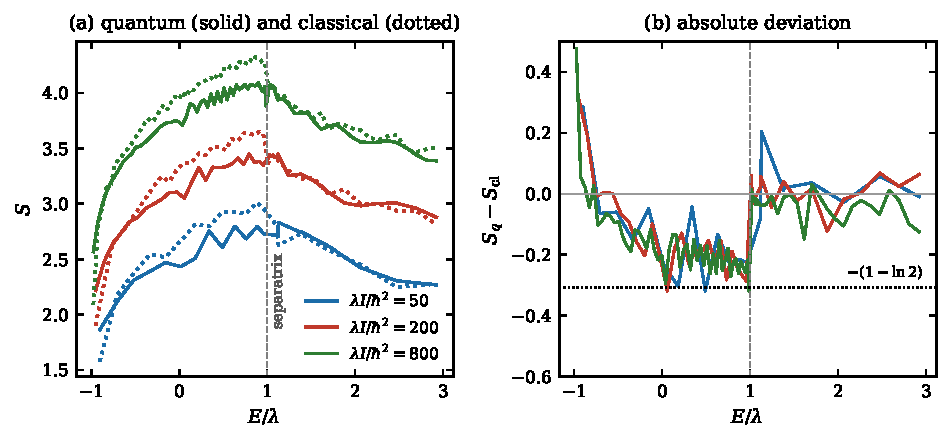
\includegraphics[width=0.92\textwidth]{fig3_separatrix.pdf}
\caption{(a) Quantum (solid) and classical coarse-grained (dotted) entropies
versus $\Erel/\lambda$ for $\lambda I/\hbar^{2}=50$, $200$, $800$; dashed line:
separatrix. (b) $S_{q}-\Scl^{\rm bin}$, with the asymptotic value $-(1-\ln2)$
dotted.}
\label{fig:separatrix}
\end{figure*}

\begin{figure*}[t]
\centering
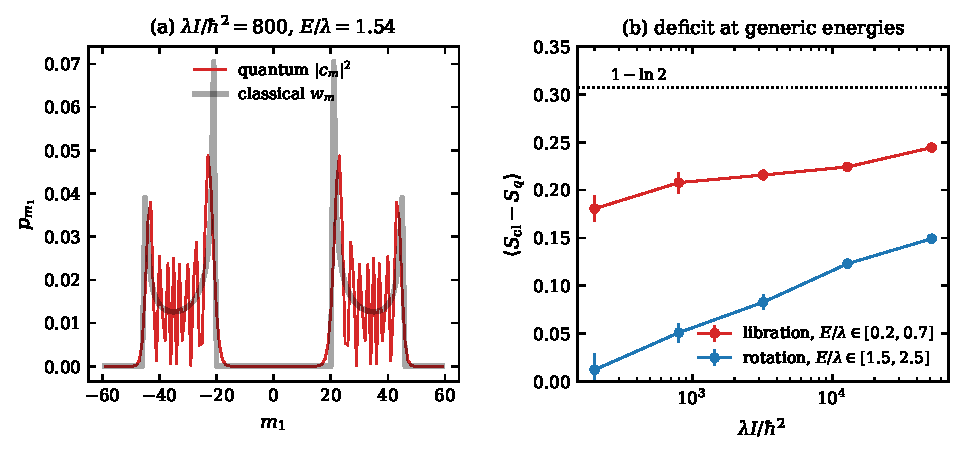
\includegraphics[width=0.92\textwidth]{fig4_fringes.pdf}
\caption{(a) Momentum distribution of rotor 1 at $\lambda I/\hbar^{2}=800$,
$\Erel/\lambda=1.54$: quantum weights (red) oscillate with full contrast about
the classical cell weights (grey), as Eq.~\eqref{eq:fringesgen} predicts.
(b) Deficit $\langle\Scl^{\rm bin}-S_{q}\rangle$ averaged over energy windows in
libration and rotation versus $\lambda$; error bars are standard errors over the
window.}
\label{fig:fringes}
\end{figure*}

Both entropies are maximal near the separatrix, at $\Erel/\lambda=1.13$, $1.12$
and $0.90$ for the three couplings, because the support of the classical
momentum distribution has its cusp maximum there. The deviation in
Fig.~\ref{fig:separatrix}(b) changes abruptly at the separatrix because the
fringe structure changes: below it the interfering branches are the two halves
of a libration orbit, above it of a rotation orbit, and new caustics appear at
$p=\pm\sqrt{I(\Erel-\lambda)}$. In the Josephson-junction realization this is
the boundary between Josephson oscillations and running-phase
motion~\cite{Smerzi97,Raghavan99}; more generally the separatrix is the
classical locus of an excited-state quantum phase
transition~\cite{CaprioCejnarIachello,Stransky,Cejnar}.

%=============================================================================
\section{Deep libration}
\label{sec:libration}
%=============================================================================

For $\lambda I/\hbar^{2}\gg1$ the ground state of $h$ is localized at
$\varphi=\pi$. With $x=\varphi-\pi$,
$h=-\lambda+p^{2}/2\mu+\tfrac12\mu\omega^{2}x^{2}-gx^{4}+\dots$ with $\mu=I/2$,
$\omega=\sqrt{2\lambda/I}$ and $g=\lambda/24$. In the harmonic approximation the
Fourier coefficients form a Gaussian in $k$ of variance
$\sigma_{0}^{2}=\mu\omega/2\hbar=\tfrac14\sqrt{2\lambda I/\hbar^{2}}$, and by
Poisson summation the Shannon entropy of a sampled Gaussian is
$\tfrac12\ln(2\pi e\sigma^{2})$ up to $O(\sigma^{2}e^{-2\pi^{2}\sigma^{2}})$. The
quartic term narrows the distribution: the virial theorem gives
$\langle p^{2}\rangle=\mu\hbar\omega/2-\hbar^{2}/16$ to first order in $g$, and
the non-Gaussian distortion does not change the entropy at first order because
$\ln\phi_{\sigma}$ is quadratic in $k$ (Appendix~\ref{app:lib}). Hence
\begin{equation}
S_{0}=\frac14\ln\frac{\lambda I}{\hbar^{2}}+\frac12\ln\frac{\pi e}{\sqrt2}
-\frac{1}{8\sqrt{2\lambda I/\hbar^{2}}}+O\!\left(\frac{\hbar^{2}}{\lambda I}\right).
\label{eq:S0}
\end{equation}
For $\lambda I/\hbar^{2}=10$, $40$, $160$, $640$, $2560$, $10240$ the ratio of the
numerical residual (after the harmonic terms) to the predicted correction is
$1.083$, $1.039$, $1.019$, $1.009$, $1.005$, $1.002$ (Fig.~\ref{fig:libration}).

\begin{figure}[t]
\centering
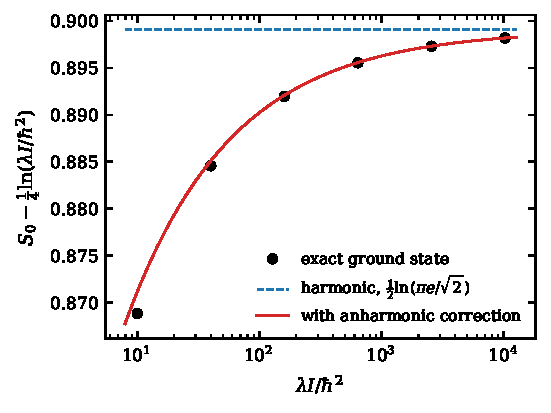
\includegraphics[width=\columnwidth]{fig5_libration.pdf}
\caption{Deep libration: $S_{0}-\tfrac14\ln(\lambda I/\hbar^{2})$ for the ground
state (points), the harmonic constant $\tfrac12\ln(\pi e/\sqrt2)$ (dashed), and
Eq.~\eqref{eq:S0} (solid).}
\label{fig:libration}
\end{figure}

%=============================================================================
\section{Wigner and Husimi distributions}
\label{sec:wigner}
%=============================================================================

We now replace the classical distribution~\eqref{eq:Wjoint} by a quantum
phase-space distribution of the eigenstate. Momenta are in units of $\hbar$.

\subsection{Wigner function: the DKS construction returns $S_{q}$}

For a rotor the Wigner function lives on $\theta\in[0,2\pi)$ and
$\ell\in\tfrac12\mathbb{Z}$~\cite{Mukunda,Bizarro,Rigas},
\begin{align}
W_{\rho}(\theta,\ell)&=\frac{1}{4\pi}\int_{-2\pi}^{2\pi}\dd\xi\,e^{-i\ell\xi}
\bra{\theta+\tfrac{\xi}{2}}\rho\ket{\theta-\tfrac{\xi}{2}}\nonumber\\
&=\frac{1}{2\pi}\sum_{m+m'=2\ell}\rho_{mm'}\,e^{i(m-m')\theta}
\label{eq:Wmm}
\end{align}
(Appendix~\ref{app:wigner}). It is real; $\sum_{\ell}W_{\rho}=\bra\theta\rho\ket\theta$;
$\int\dd\theta\,W_{\rho}=\rho_{\ell\ell}$ for integer $\ell$ and $0$ for
half-integer $\ell$; and $\Tr\rho\sigma=2\pi\sum_{\ell}\int\dd\theta\,W_{\rho}
W_{\sigma}$. For two rotors, integrating the two-rotor Wigner function over
$(\theta_{2},\ell_{2})$ is the partial trace:
$\sum_{\ell_{2}}\int\dd\theta_{2}\,W=W_{\rho_{1}}$. For an eigenstate,
\begin{multline}
W(\theta_{1},\ell_{1};\theta_{2},\ell_{2})\\
=\frac{1}{2\pi}\,\delta_{\ell_{1}+\ell_{2},M}\,
W_{\rm rel}\big(\theta_{1}-\theta_{2},\,\ell_{1}-\tfrac M2\big),
\label{eq:Wfactor}
\end{multline}
with $W_{\rm rel}(\varphi,\ell)=(2\pi)^{-1}\sum_{k+k'=2\ell}c_{k}\bar c_{k'}
e^{i(k-k')\varphi}$ the Wigner function of $u(\varphi)$. The microcanonical
distribution has the same skeleton,
$W_{\rm cl}=(2\pi)^{-1}\delta(J-p_{1}-p_{2})\,\delta(\Erel-H_{\rm rel})/4B$: the
only difference is $W_{\rm rel}$ versus the microcanonical density on the
pendulum level set.

Carrying out the DKS construction with $W$ in place of $W_{\rm cl}$, the reduced
Wigner function is $W_{1}=p_{k}/2\pi$ at $\ell_{1}=\tfrac M2+k$ and zero on the
other half-integer rows. It is non-negative (because $\rho_{1}$ is diagonal) and
its Boltzmann entropy with cell $h$ is
\begin{equation}
-\sum_{\ell_{1}}\int_{0}^{2\pi}\dd\theta_{1}\,W_{1}\ln(2\pi W_{1})
=-\sum_{k}p_{k}\ln p_{k}=S_{q},
\label{eq:SWig}
\end{equation}
identically, for every eigenstate and coupling. Replacing the classical
distribution by the Wigner function gives the quantum answer, not a classical
one.

\subsection{The deficit lives in the chord terms}

Figure~\ref{fig:wigner} shows $W_{\rm rel}$ for a librating and a rotating level.
As for any one-dimensional eigenstate~\cite{Berry77,OzorioRep}, $W_{\rm rel}$ is
large on the classical curve, with an Airy profile across it, and oscillates
inside: a point $(\varphi,\ell)$ receives a contribution from each chord of the
curve centered on it, with phase equal to the enclosed symplectic area over
$\hbar$. The negativity volume~\cite{Kenfack} $\sum_{\ell}\int|W_{\rm rel}|-1$ is
$5.86$ and $5.43$ for the two states shown. Averaged over regions large compared
with $\hbar$ but classically small, the chord terms cancel and $W_{\rm rel}$
reduces to the microcanonical density~\cite{Berry77,Voros}.

\begin{figure*}[t]
\centering
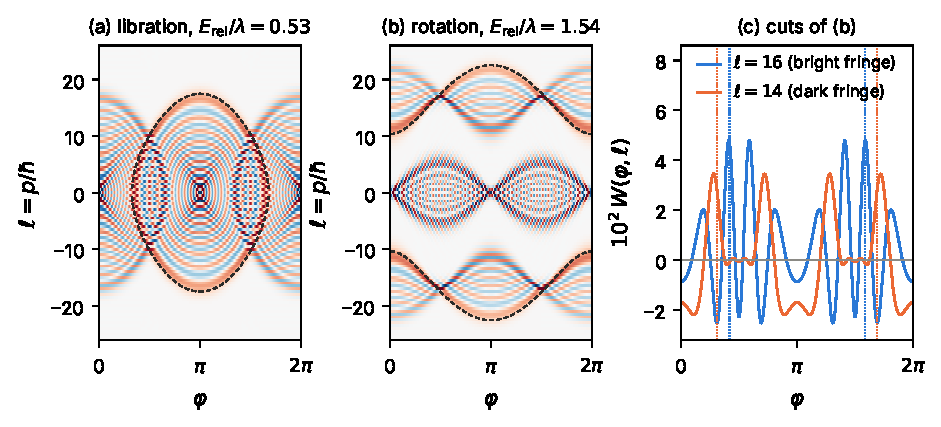
\includegraphics[width=0.92\textwidth]{fig6_wigner.pdf}
\caption{Relative Wigner function $W_{\rm rel}(\varphi,\ell)$ at
$\lambda I/\hbar^{2}=200$ (red positive, blue negative; integer and half-integer
rows). (a) Librating level, $\Erel/\lambda=0.53$. (b) Rotating level,
$\Erel/\lambda=1.54$, odd parity; the band near $\ell=0$ is the interference of
the two counter-rotating tori. Dashed: classical curve. (c) Cuts of (b) at
$\ell=16$ (bright fringe of $p_{\ell}$) and $\ell=14$ (dark fringe); dotted lines:
classical angles $\pm\phi_{\ell}$. The oscillations away from them are the chord
terms that survive integration over $\varphi$.}
\label{fig:wigner}
\end{figure*}

Integrating $W_{\rm rel}$ over $\varphi$ at integer $\ell$ collects (a) the two
points of the classical curve at momentum $\ell$, $\varphi=\pm\phi_{\ell}$, which
give the classical weight $w_{\ell}$, and (b) the horizontal chord joining them,
centered on $\varphi=0$ and $\pi$, which gives $w_{\ell}\cos\Phi_{\ell}$. At
$\ell=14$ in Fig.~\ref{fig:wigner}(c), windows of half-width $0.35$ around
$\pm\phi_{\ell}$ contribute $+0.022$, around $0$ and $\pi$ $-0.027$, and the total
is $p_{14}=7\times10^{-4}$: a dark fringe. On half-integer rows the chord
contributions at $0$ and $\pi$ cancel ($\mp0.012$ at $\ell=16.5$). Smoothing
before marginalizing gives the classical distribution; marginalizing first keeps
the chord terms. \emph{The constant $1-\ln2$ is the entropy carried by the chord
terms of the Wigner function.}

\subsection{Husimi function and Wehrl entropy}

The Husimi function removes chord terms by smoothing over a coherent state. On
the circle we use~\cite{KRP,GonzalezOlmo}
\begin{equation}
\ket{\theta,\ell}=\sum_{m}\sqrt{g_{\sigma}(m-\ell)}\,e^{-im\theta}\ket m,\quad
g_{\sigma}(x)=\frac{e^{-x^{2}/2\sigma^{2}}}{\sqrt{2\pi}\,\sigma},
\label{eq:cs}
\end{equation}
with $\ell\in\mathbb{R}$, momentum width $\sigma$ and angular width $1/2\sigma$.
The resolution of identity
$\int\frac{\dd\theta}{2\pi}\dd\ell\,\ketbra{\theta,\ell}{\theta,\ell}=\mathbb{1}$
holds exactly with cell $h$, and the norm is $1$ up to
$2e^{-2\pi^{2}\sigma^{2}}$ ($1.4\%$ at $\sigma=\tfrac12$). For the
state~\eqref{eq:Smathieu} the Husimi function is
$Q(\ell)=\sum_{m}p_{m}g_{\sigma}(\ell-m)$, independent of $\theta$, and the Wehrl
entropy~\cite{Wehrl,Wehrl79} is $\SW=-\int\dd\ell\,Q\ln Q$. Applied to the
classical density, the same smoothing gives $\SW[w]\to\Scl$ as $\sigma\to0$.
Jensen's inequality (the Berezin--Lieb bound~\cite{Berezin,Lieb}) and
$h(M+Z)\le H(M)+h(Z)$~\cite{CoverThomas} give
\begin{equation}
S_{q}-2e^{-2\pi^{2}\sigma^{2}}\lesssim\SW\le S_{q}+\tfrac12\ln(2\pi e\sigma^{2}).
\label{eq:bounds}
\end{equation}

\emph{Deep rotation in closed form.} Over a stretch of cells where $w$ is nearly
constant and $\Phi_{j}\simeq\Phi_{0}+\kappa j$ with $\kappa=-2\beta$, Poisson
summation gives $\sum_{j}e^{i\kappa j}g_{\sigma}(x-j)=\sum_{r}
e^{i(\kappa+2\pi r)x}e^{-\sigma^{2}(\kappa+2\pi r)^{2}/2}$. For $\sigma\gtrsim1$
only the alias nearest zero survives, and
\begin{equation}
\begin{gathered}
Q\simeq w\left[1+A\cos\tilde\Phi\right],\qquad A=e^{-\sigma^{2}d^{2}/2},\\
d=\min(2\beta,2\pi-2\beta).
\end{gathered}
\label{eq:Qfringe}
\end{equation}
Smoothing reduces the fringe contrast from $1$ to $A$ without removing the
fringes. Averaging over the fast phase,
$\SW\simeq\Scl-\int w\,f(A)$, with the contrast function
(Appendix~\ref{app:integrals})
\begin{equation}
\begin{split}
f(A)&=\big\langle(1+A\cos\Phi)\ln(1+A\cos\Phi)\big\rangle\\
&=\ln\frac{1+\sqrt{1-A^{2}}}{2}+1-\sqrt{1-A^{2}},
\end{split}
\label{eq:fA}
\end{equation}
which gives $f(1)=1-\ln2$. Since the arcsine weight is uniform in $\beta$,
\begin{equation}
\begin{gathered}
\SW-S_{q}=\left(1-\ln2\right)-D(\sigma),\\
D(\sigma)=\frac{2}{\pi}\int_{0}^{\pi/2}f\big(e^{-2\sigma^{2}\beta^{2}}\big)\,\dd\beta .
\end{gathered}
\label{eq:Dsigma}
\end{equation}
Both Eq.~\eqref{eq:fringesgen} and Eq.~\eqref{eq:Qfringe} fail near the
caustics, but there $A\to1$ and the integrand $f(1)-f(A)$ of $\SW-S_{q}$
vanishes, so Eq.~\eqref{eq:Dsigma} holds without the $\gamma^{-1/3}$ correction.
For $\sigma\gg1$, expanding $f$ in powers of $A^{2}$,
\begin{equation}
\begin{gathered}
D(\sigma)\simeq\frac{c_{1}}{\sigma},\\
c_{1}=\frac{1}{2\sqrt\pi}\sum_{n\ge1}\frac{\binom{2n}{n}}{4^{n}\,2n(2n-1)\sqrt n}=0.080171,
\end{gathered}
\label{eq:c1}
\end{equation}
accurate to $10^{-5}$ for $\sigma\ge1$. Table~\ref{tab:husimi_rot} tests
Eq.~\eqref{eq:Dsigma} (column ``pred.'') against the Bessel weights. At $\gamma=10^{4}$ the agreement
is within $0.001$ for $1\le\sigma\le4$, and $\SW-S_{q}$ is the same at
$\gamma=10^{3}$ and $10^{4}$ to $0.004$ although $\Scl-S_{q}$ changes from $0.212$ to
$0.263$. At $\sigma=\tfrac12$ a second alias lowers the result by $0.003$; at
$\gamma\le100$ the larger widths resolve the band itself.

\begin{table}[t]
\caption{Wehrl entropy of the deep-rotation weights $J_{j}^{2}(\gamma)$ against
Eq.~\eqref{eq:Dsigma}; $\SW[w]$ is the arcsine law smoothed with the same
$\sigma$, and $\Scl=\ln(\pi\gamma/2)$.}
\label{tab:husimi_rot}
\footnotesize
\setlength{\tabcolsep}{1pt}
\begin{ruledtabular}
\begin{tabular}{rrcccc}
$\gamma$ & $\sigma$ & $\SW-S_{q}$ & pred. & $\SW-\Scl$ &
$\SW[w]-\SW$\\
\hline
$10^{2}$ & $0.5$ & 0.1406 & 0.1502 & $0.0453$ & $0.0364$\\
         & $1$   & 0.2218 & 0.2267 & $0.1265$ & $-0.0110$\\
         & $2$   & 0.2713 & 0.2668 & $0.1760$ & $-0.0127$\\
         & $4$   & 0.3300 & 0.2868 & $0.2347$ & $-0.0040$\\
$10^{3}$ & $0.5$ & 0.1468 & 0.1502 & $-0.0654$ & $0.0912$\\
         & $1$   & 0.2274 & 0.2267 & $0.0152$ & $0.0213$\\
         & $2$   & 0.2680 & 0.2668 & $0.0558$ & $-0.0041$\\
         & $4$   & 0.2916 & 0.2868 & $0.0795$ & $-0.0064$\\
$10^{4}$ & $0.5$ & 0.1468 & 0.1502 & $-0.1165$ & $0.1247$\\
         & $1$   & 0.2274 & 0.2267 & $-0.0359$ & $0.0475$\\
         & $2$   & 0.2675 & 0.2668 & $0.0042$ & $0.0121$\\
         & $4$   & 0.2877 & 0.2868 & $0.0244$ & $-0.0013$\\
\end{tabular}
\end{ruledtabular}
\end{table}

Thus, at fixed $\sigma$ and $\gamma\to\infty$,
\begin{equation}
\SW-\Scl\;\to\;-D(\sigma)\simeq-0.080/\sigma :
\label{eq:SWScl}
\end{equation}
the Husimi entropy does not converge to the classical one. The classical value is
reached only for $1\ll\sigma\ll\gamma$, and only algebraically, because fringes
of every wavenumber down to zero exist near the band edges and a Gaussian of any
width leaves the slowest intact [Fig.~\ref{fig:husimi}(a)].

\emph{Generic energies.} The local fringe wavenumber is $2\phi_{k}$, and the same
argument gives $\SW-S_{q}\simeq(1-\ln2)-\langle f(e^{-\sigma^{2}d(2\phi)^{2}/2})
\rangle_{\rm orbit}$, which agrees with the numerics to within $0.03$ for
$\sigma\le1$ in the windows of Sec.~\ref{sec:compare}
(Table~\ref{tab:husimi_gen}). The fair comparison smooths quantum and classical
distributions with the same coherent state. For $\sigma=1$ the two Wehrl entropies
then agree to within $0.04$, and for $\sigma=2$ to within $0.015$, at every level
with $-0.5<\Erel/\lambda<0.8$ or $1.2<\Erel/\lambda<3$ at
$\lambda I/\hbar^{2}=200$ and $800$ [Fig.~\ref{fig:husimi}(b)], compared with an
unsmoothed deficit of about $0.2$ in libration. But the agreement is achieved by
moving both entropies: $\SW[w]$ exceeds $\Scl$ by $0.1$--$0.7$, depending on
$\sigma$ and the width of the band.

\begin{table*}[t]
\caption{Window averages ($0.2\le\Erel/\lambda\le0.7$ libration,
$1.5\le\Erel/\lambda\le2.5$ rotation), all levels of sector $M=0$.}
\label{tab:husimi_gen}
\small
\setlength{\tabcolsep}{6pt}
\begin{ruledtabular}
\begin{tabular}{lccccccc}
$\lambda I/\hbar^{2}$ & regime & $\Scl^{\rm bin}-S_{q}$ & $\sigma$ &
$\SW-S_{q}$ & $(1-\ln2)-\langle f\rangle_{\rm orbit}$ & $\SW[w]-\SW$ & $\SW[w]-\Scl$\\
\hline
200 & libration & 0.180 & 0.5 & 0.193 & 0.204 & $\phantom{-}0.025$ & 0.147\\
    &      &       & 1   & 0.284 & 0.270 & $-0.007$ & 0.207\\
    &      &       & 2   & 0.364 & 0.289 & $-0.002$ & 0.292\\
200 & rotation & 0.012 & 0.5 & 0.146 & 0.146 & $-0.046$ & 0.361\\
    &      &       & 1   & 0.273 & 0.223 & $-0.026$ & 0.508\\
    &      &       & 2   & 0.459 & 0.264 & $-0.007$ & 0.713\\
800 & libration & 0.208 & 0.5 & 0.202 & 0.204 & $\phantom{-}0.031$ & 0.104\\
    &      &       & 1   & 0.284 & 0.270 & $-0.008$ & 0.147\\
    &      &       & 2   & 0.339 & 0.289 & $-0.003$ & 0.207\\
800 & rotation & 0.051 & 0.5 & 0.144 & 0.146 & $-0.030$ & 0.256\\
    &      &       & 1   & 0.246 & 0.223 & $-0.027$ & 0.361\\
    &      &       & 2   & 0.374 & 0.264 & $-0.009$ & 0.508\\
\end{tabular}
\end{ruledtabular}
\end{table*}

\begin{figure*}[t]
\centering
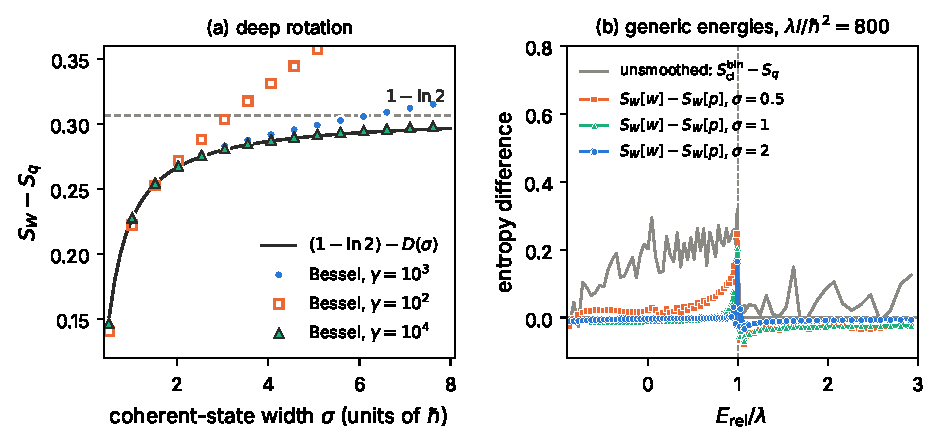
\includegraphics[width=0.92\textwidth]{fig7_husimi.pdf}
\caption{(a) Deep rotation: excess of the Wehrl over the von Neumann entropy
versus coherent-state width, Eq.~\eqref{eq:Dsigma} (solid), and Bessel weights at
$\gamma=10^{2},10^{3},10^{4}$ (symbols). The full deficit $1-\ln2$ (dashed) is
recovered only as $\sigma\to\infty$. (b) Generic energies at
$\lambda I/\hbar^{2}=800$: difference between the Wehrl entropies of the
classical and quantum momentum distributions for $\sigma=0.5,1,2$, and the
unsmoothed difference $\Scl^{\rm bin}-S_{q}$ (grey). Dashed line: separatrix.}
\label{fig:husimi}
\end{figure*}

The coherent-state width is not fixed by the problem. It therefore takes over
the role of the cell $\Delta$ in the oscillator problem: a parameter outside the
classical theory whose choice decides the constant term. The cell itself stays
fixed at $h$ by the resolution of identity. The width $\sigma_{0}\propto
(\lambda I/\hbar^{2})^{1/4}$ of the pendulum ground state is a natural choice,
for which $D(\sigma_{0})\to0$ in the semiclassical limit, but only as
$(\lambda I/\hbar^{2})^{-1/4}$, and the choice is a convention.

%=============================================================================
\section{Conclusions}
\label{sec:disc}
%=============================================================================

For two coupled rotors, conservation of total angular momentum fixes both the
Schmidt basis and the phase-space cell, so the classical--quantum comparison of
entanglement entropy proposed in Ref.~\cite{DKS} can be made with nothing to
adjust. The leading logarithms agree, as for oscillators, but the quantum entropy
lies below the classical one by the universal constant $1-\ln2$, the entropy of
full-contrast interference between the two classical branches compatible with one
observed momentum. In phase space this interference is the chord structure of the
Wigner function. Replacing the classical distribution by the Wigner function
gives back the von Neumann entropy identically; replacing it by the Husimi
function gives an intermediate value with a closed-form dependence on the
coherent-state width, $(1-\ln2)-D(\sigma)$, $D\simeq0.080/\sigma$. No phase-space
route reproduces the entanglement entropy, constant term included, without one
conventional parameter: a cell for the oscillators, a coherent-state width for
the Husimi function, or, when both are fixed as here, an explicit correction
$1-\ln2$.

At weak coupling the entropy is controlled by the $O(\lambda^{2})$ normalization
of the perturbed state; at the separatrix both entropies peak; in deep libration
the entropy is $\tfrac14\ln(\lambda I/\hbar^{2})+\tfrac12\ln(\pi e/\sqrt2)$ up to
an anharmonic correction verified to three digits.

In the bosonic Josephson junction the Schmidt weights are the atom-number
distribution of one well at fixed total number, so the entropies compared here
are, in principle, number-statistics measurements, and the separatrix is the
onset of running-phase motion~\cite{Albiez05,GatiOberthaler}. Natural extensions are unequal moments of
inertia (exchange symmetry broken, $J$ conserved), $N>2$ rotors, where the
relative motion becomes non-integrable, and quenches of $\lambda$ across the
separatrix.

\begin{acknowledgments}
[To be completed.]
\end{acknowledgments}

\appendix

%=============================================================================
\section{Perturbation theory}
\label{app:pt}
%=============================================================================

Write $H=H_{0}+V$ and expand
$\ket{\widetilde\Psi}=\ket0+\ket{\psi^{(1)}}+\ket{\psi^{(2)}}+\dots$ with
intermediate normalization $\braket0{\psi^{(k)}}=0$. Then $E^{(1)}=V_{00}$,
$\ket{\psi^{(1)}}=\sum_{k\ne0}V_{k0}\ket k/(E_{0}-E_{k})$,
$E^{(2)}=\sum_{k\ne0}|V_{k0}|^{2}/(E_{0}-E_{k})$, and
\begin{equation}
\ket{\psi^{(2)}}=\sum_{k,l\ne0}\frac{V_{kl}V_{l0}\ket k}{(E_{0}-E_{k})(E_{0}-E_{l})}
-\sum_{k\ne0}\frac{V_{00}V_{k0}\ket k}{(E_{0}-E_{k})^{2}}.
\end{equation}
From Eq.~\eqref{eq:V}, $V_{00}=0$ and the only non-zero $V_{k0}$ are
$V_{\pm,0}=\lambda/2$ for $\ket\pm=\ket{m_{1}\pm1,m_{2}\mp1}$, with
$E_{0}-E_{\pm}=\mp\hbar^{2}(n\pm1)/I$ and, for $\ket{\pm\pm}=\ket{m_{1}\pm2,m_{2}\mp2}$,
$E_{0}-E_{\pm\pm}=\mp2\hbar^{2}(n\pm2)/I$. These give Eq.~\eqref{eq:E2}, the
amplitudes $c_{\pm}$, and $c_{\pm\pm}$ quoted in Sec.~\ref{sec:weak}; the state
$\ket0$ itself is excluded from the second-order sum. The normalized state is
$\mathcal{N}\ket{\widetilde\Psi}$ with $\mathcal{N}^{-2}=1+\epsp+\epsm+O(\lambda^{4})$.

To second order, $\rho=\ketbra\Psi\Psi$ contains thirteen entries: the
$\ketbra00$ element $1-\epsp-\epsm$, four first-order coherences
$c_{\pm}(\ketbra\pm0+{\rm h.c.})$, the populations $\varepsilon_{\pm}$, the
coherence $c_{+}c_{-}(\ketbra+-+{\rm h.c.})$, and four entries
$c_{\pm\pm}(\ketbra{\pm\pm}0+{\rm h.c.})$. One checks
$\Tr\rho=1$ and $\Tr\rho^{2}=(1-\varepsilon)^{2}+2\varepsilon+O(\lambda^{4})=1$
with $\varepsilon=\epsp+\epsm$; both fail if the normalization term is omitted.
Under the partial trace, $\Tr_{2}\ketbra{a,b}{c,d}=\delta_{bd}\ketbra ac$, every
coherence connects different rotor-2 labels and drops out, leaving
Eq.~\eqref{eq:rho1}; the $O(\lambda^{3})$ terms of $\rho$ are also off-diagonal
in $m_{2}$, so the error is $O(\lambda^{4})$.

%=============================================================================
\section{Integrals}
\label{app:integrals}
%=============================================================================

\emph{Band integrals.} With $\Erel-p^{2}/I=\lambda\cos u$,
$B=\tfrac{\sqrt I}{2}\int\dd u\,(\Erel-\lambda\cos u)^{-1/2}$. In rotation,
$u=\pi-2t$ gives $\Erel-\lambda\cos u=(\Erel+\lambda)(1-k^{2}\sin^{2}t)$ with
$k^{2}=2\lambda/(\Erel+\lambda)$. In libration, $v=\pi-u$ and
$\sin(v/2)=\kappa\sin t$ with $\kappa^{2}=(\Erel+\lambda)/2\lambda$ give
$\Erel+\lambda\cos v=(\Erel+\lambda)\cos^{2}t$ and
$\dd v=2\kappa\cos t\,\dd t/(1-\kappa^{2}\sin^{2}t)^{1/2}$. Both lead to
Eq.~\eqref{eq:B}, and both parametrize the orbit uniformly in time,
$\dd t_{\rm orbit}\propto\dd t/(1-k^{2}\sin^{2}t)^{1/2}$, which we use to sample
the classical density.

\emph{Arcsine entropy and phase average.} From
$\int_{0}^{\pi}\ln\sin u\,\dd u=-\pi\ln2$ and $j=\gamma\cos\beta$ (so
$w\,\dd j=\dd\beta/\pi$), $-\int w\ln w=\ln\pi+\ln\gamma-\ln2$. With
$1+\cos\Phi=2\cos^{2}(\Phi/2)$, $\langle\ln(1+\cos\Phi)\rangle=-\ln2$, and
integrating by parts, $\langle\cos\Phi\ln(1+\cos\Phi)\rangle=
\langle\sin^{2}\Phi/(1+\cos\Phi)\rangle=1$; the sum is $1-\ln2$.

\emph{Contrast function.} With $s=\sqrt{1-A^{2}}$,
$\langle\ln(1+A\cos\Phi)\rangle=\ln[(1+s)/2]$~\cite{GR}, and integrating by
parts, $\langle\cos\Phi\ln(1+A\cos\Phi)\rangle=A\langle\sin^{2}\Phi/u\rangle$
with $u=1+A\cos\Phi$. Using $\sin^{2}\Phi=(A^{2}-1+2u-u^{2})/A^{2}$,
$\langle u^{-1}\rangle=1/s$ and $\langle u\rangle=1$, this is $(1-s)/A$, which
gives Eq.~\eqref{eq:fA}. Alternatively, from
$(1+y)\ln(1+y)=y+\sum_{k\ge2}(-1)^{k}y^{k}/k(k-1)$ and
$\langle\cos^{2n}\Phi\rangle=\binom{2n}{n}4^{-n}$,
$f(A)=\sum_{n\ge1}\binom{2n}{n}A^{2n}/[4^{n}2n(2n-1)]$; with
$\int_{0}^{\infty}e^{-4n\sigma^{2}\beta^{2}}\dd\beta=\sqrt\pi/(4\sigma\sqrt n)$ this
gives Eq.~\eqref{eq:c1}.

%=============================================================================
\section{Deep libration}
\label{app:lib}
%=============================================================================

For $p_{k}\propto e^{-k^{2}/2\sigma^{2}}$ on the integers, Poisson summation gives
$Z=\sqrt{2\pi}\sigma[1+2\sum_{r\ge1}e^{-2\pi^{2}\sigma^{2}r^{2}}]$ and
$\langle k^{2}\rangle=\sigma^{2}[1+O(\sigma^{2}e^{-2\pi^{2}\sigma^{2}})]$, so
$S=\ln Z+\langle k^{2}\rangle/2\sigma^{2}=\tfrac12\ln(2\pi e\sigma^{2})$ up to
exponentially small terms. The virial theorem $2\langle T\rangle=\langle xV'\rangle$
with $V=\tfrac12\mu\omega^{2}x^{2}-gx^{4}$ gives
$\langle T\rangle=\tfrac12(E-\langle gx^{4}\rangle)$; to first order
$E=\tfrac12\hbar\omega-g\langle x^{4}\rangle_{0}$ and
$\langle x^{4}\rangle_{0}=3\hbar^{2}/4\mu^{2}\omega^{2}$, so
$\langle p^{2}\rangle=\mu\hbar\omega/2-3g\hbar^{2}/2\mu\omega^{2}
=\mu\hbar\omega/2-\hbar^{2}/16$. If $p=\phi_{\sigma}(1+\epsilon\eta)$ with
$\phi_{\sigma}$ the Gaussian of the exact variance, $\eta$ is orthogonal to $1$,
$k$, $k^{2}$ and the entropy changes only at $O(\epsilon^{2})$. Expanding
$\tfrac12\ln[2\pi e(\sigma_{0}^{2}-\tfrac1{16})]$ gives Eq.~\eqref{eq:S0}.

%=============================================================================
\section{Wigner function on the circle}
\label{app:wigner}
%=============================================================================

The kernel $\bra{\theta+\xi/2}\rho\ket{\theta-\xi/2}=(2\pi)^{-1}\sum_{mm'}
\rho_{mm'}e^{i(m-m')\theta}e^{i(m+m')\xi/2}$ is $4\pi$-periodic in $\xi$, so its
Fourier variable $\ell$ runs over $\tfrac12\mathbb{Z}$; using
$\int_{-2\pi}^{2\pi}e^{is\xi}\dd\xi=4\pi\delta_{s0}$ for $s\in\tfrac12\mathbb{Z}$
gives Eq.~\eqref{eq:Wmm}. For two rotors,
$W=(2\pi)^{-2}\sum\rho_{m_{1}m_{2};m_{1}'m_{2}'}
e^{i(m_{1}-m_{1}')\theta_{1}+i(m_{2}-m_{2}')\theta_{2}}$ with
$m_{i}+m_{i}'=2\ell_{i}$; the $\theta_{2}$ integral sets $m_{2}'=m_{2}$ and the
sum over $\ell_{2}$ sums over $m_{2}$, giving $W_{\rho_{1}}$. For an eigenstate,
$\rho_{m_{1}m_{2};m_{1}'m_{2}'}=c_{k}\bar c_{k'}$ with $2\ell_{1}=M+k+k'$,
$2\ell_{2}=M-k-k'$ and phase $(k-k')(\theta_{1}-\theta_{2})$, which is
Eq.~\eqref{eq:Wfactor}. For the classical distribution,
$\int\dd\varphi\,\dd p\,\delta(\Erel-H_{\rm rel})=4B$ and $\mathcal{C}=1/8\pi B$.

%=============================================================================
\section{Numerical methods and checks}
\label{app:num}
%=============================================================================

We use $\hbar=I=1$ and the sector $M=0$. The pendulum is diagonalized in the
parity sectors with bases $\{\chi_{0},(\chi_{k}+\chi_{-k})/\sqrt2\}$ (where
$\bra{\chi_{0}}h\,(\chi_{1}+\chi_{-1})/\sqrt2\rangle=\lambda/\sqrt2$) and
$\{(\chi_{k}-\chi_{-k})/\sqrt2\}$, $\chi_{k}=e^{ik\varphi}/\sqrt{2\pi}$, with
truncation $|k|\le8\sqrt\lambda+150$. Classical cell weights use adaptive
quadrature with the band-edge singularities supplied; Bessel sums run over
$|j|\le\gamma+40\gamma^{1/3}+50$. Wehrl entropies of discrete weights are
computed by convolution on $\ge10/\sigma$ points per cell; those of the classical
density by sampling the orbit uniformly in time ($2\times10^{5}$ points),
histogramming at resolution $0.01$ and convolving. Table~\ref{tab:checks} lists
the checks quoted in the text.

\begin{table}[h]
\caption{Analytic results against exact numerics ($\hbar=I=1$). Perturbative
checks at $n=7$ ($m_{1}=9,m_{2}=2$), $\lambda=0.02$; Mathieu checks at
$q=14.6$; Wigner checks at $\lambda=200$, $\Erel/\lambda=1.54$.}
\label{tab:checks}
\footnotesize
\setlength{\tabcolsep}{2pt}
\begin{ruledtabular}
\begin{tabular}{lll}
quantity & analytic & numerical\\
\hline
$c_{+}$ & $-0.0012500$ & $-0.0012500$\\
$c_{-}$ & $0.0016667$ & $0.0016667$\\
$c_{++}$ & $6.944444\times10^{-7}$ & $6.944456\times10^{-7}$\\
$c_{--}$ & $1.666667\times10^{-6}$ & $1.666669\times10^{-6}$\\
$E^{(2)}$, Eq.~\eqref{eq:E2} & $4.166667\times10^{-6}$ & $4.166668\times10^{-6}$\\
$S$, $n=0$, Eq.~\eqref{eq:Sweak} & 0.0020420 & 0.0020411\\
$S$, $n=30$, $\lambda=0.05$ & $2.1084\times10^{-5}$ & $2.1146\times10^{-5}$\\
$M=0$ lowest level vs $a_{0}/4$ & $-5.4542890$ & $-5.4542890$\\
$M=1$ lowest level vs $b_{1}/4$ & $-5.4542787$ & $-5.4542787$\\
$B$, $\Erel=300$, $\lambda=100$ & 0.0927037 & 0.0927037\\
$B$, $\Erel=60$, $\lambda=100$ & 0.1596085 & 0.1596085\\
$p_{0}$, $n=400$, $\gamma=5$ vs $J_{0}^{2}(5)$ & 0.0315406 & 0.0314917\\
$\Scl^{\rm bin}-S_{q}$, $\gamma=10^{6}$ vs $1-\ln2$ & 0.3068528 & 0.2978385\\
$S_{0}$, $\lambda=10240$, Eq.~\eqref{eq:S0} & 3.2067189 & 3.2067169\\
$\sum_{\ell}\int W_{\rm rel}$ & 1 & 1.000000000000\\
$\max_{\ell\in\mathbb{Z}}|\int W_{\rm rel}-p_{\ell}|$ & 0 & $3.8\times10^{-17}$\\
$\max_{\ell\in\mathbb{Z}+\frac12}|\int W_{\rm rel}|$ & 0 & $3.0\times10^{-17}$\\
$\sigma D(\sigma)$ at $\sigma=8$ vs $c_{1}$ & 0.080171 & 0.080171\\
$\SW-S_{q}$, $\gamma=10^{4}$, $\sigma=1$ & 0.2267 & 0.2274\\
\end{tabular}
\end{ruledtabular}
\end{table}

\begin{thebibliography}{99}

\bibitem{DKS} H.~Duan, A.~Kovner, and V.~V.~Skokov, Classical entanglement and
entropy, arXiv:2301.05735.
\bibitem{KharzeevLevin} D.~E.~Kharzeev and E.~M.~Levin, Phys.\ Rev.\ D
\textbf{95}, 114008 (2017).
\bibitem{Kutak} K.~Kutak, Phys.\ Lett.\ B \textbf{705}, 217 (2011).
\bibitem{Hagiwara} Y.~Hagiwara, Y.~Hatta, B.-W.~Xiao, and F.~Yuan, Phys.\ Rev.\ D
\textbf{97}, 094029 (2018).
\bibitem{Smerzi97} A.~Smerzi, S.~Fantoni, S.~Giovanazzi, and S.~R.~Shenoy,
Phys.\ Rev.\ Lett.\ \textbf{79}, 4950 (1997).
\bibitem{Raghavan99} S.~Raghavan, A.~Smerzi, S.~Fantoni, and S.~R.~Shenoy,
Phys.\ Rev.\ A \textbf{59}, 620 (1999).
\bibitem{GatiOberthaler} R.~Gati and M.~K.~Oberthaler, J.\ Phys.\ B \textbf{40},
R61 (2007).
\bibitem{FazioReview} R.~Fazio and H.~van der Zant, Phys.\ Rep.\ \textbf{355},
235 (2001).
\bibitem{Albiez05} M.~Albiez, R.~Gati, J.~F\"olling, S.~Hunsmann, M.~Cristiani,
and M.~K.~Oberthaler, Phys.\ Rev.\ Lett.\ \textbf{95}, 010402 (2005).
\bibitem{Hines03} A.~P.~Hines, R.~H.~McKenzie, and G.~J.~Milburn, Phys.\ Rev.\ A
\textbf{67}, 013609 (2003).
\bibitem{Wehrl} A.~Wehrl, Rev.\ Mod.\ Phys.\ \textbf{50}, 221 (1978).
\bibitem{PSinfo1} arXiv:2410.16338 [full reference to be completed].
\bibitem{PSinfo2} arXiv:2606.02656 [full reference to be completed].
\bibitem{DLMF28} NIST Digital Library of Mathematical Functions, Chap.~28,
\url{https://dlmf.nist.gov/28}.
\bibitem{Wannier} G.~H.~Wannier, Phys.\ Rev.\ \textbf{117}, 432 (1960).
\bibitem{Fukuyama} H.~Fukuyama, R.~A.~Bari, and H.~C.~Fogedby, Phys.\ Rev.\ B
\textbf{8}, 5579 (1973).
\bibitem{DLMF10} NIST Digital Library of Mathematical Functions, \S10.19,
\url{https://dlmf.nist.gov/10.19}.
\bibitem{CaprioCejnarIachello} M.~A.~Caprio, P.~Cejnar, and F.~Iachello,
Ann.\ Phys.\ (NY) \textbf{323}, 1106 (2008).
\bibitem{Stransky} P.~Str\'ansk\'y, M.~Macek, and P.~Cejnar, Ann.\ Phys.\ (NY)
\textbf{345}, 73 (2014).
\bibitem{Cejnar} P.~Cejnar, P.~Str\'ansk\'y, M.~Macek, and M.~Kloc, J.\ Phys.\ A
\textbf{54}, 133001 (2021).
\bibitem{Mukunda} N.~Mukunda, Am.\ J.\ Phys.\ \textbf{47}, 182 (1979).
\bibitem{Bizarro} J.~P.~Bizarro, Phys.\ Rev.\ A \textbf{49}, 3255 (1994).
\bibitem{Rigas} I.~Rigas, L.~L.~S\'anchez-Soto, A.~B.~Klimov,
J.~\v{R}eh\'a\v{c}ek, and Z.~Hradil, Ann.\ Phys.\ (NY) \textbf{326}, 426 (2011).
\bibitem{Berry77} M.~V.~Berry, Phil.\ Trans.\ R.\ Soc.\ Lond.\ A \textbf{287},
237 (1977).
\bibitem{OzorioRep} A.~M.~Ozorio de Almeida, Phys.\ Rep.\ \textbf{295}, 265 (1998).
\bibitem{Kenfack} A.~Kenfack and K.~\.Zyczkowski, J.\ Opt.\ B \textbf{6}, 396 (2004).
\bibitem{Voros} A.~Voros, Ann.\ Inst.\ H.\ Poincar\'e A \textbf{24}, 31 (1976).
\bibitem{KRP} K.~Kowalski, J.~Rembieli\'nski, and L.~C.~Papaloucas, J.\ Phys.\ A
\textbf{29}, 4149 (1996).
\bibitem{GonzalezOlmo} J.~A.~Gonz\'alez and M.~A.~del Olmo, J.\ Phys.\ A
\textbf{31}, 8841 (1998).
\bibitem{Wehrl79} A.~Wehrl, Rep.\ Math.\ Phys.\ \textbf{16}, 353 (1979).
\bibitem{Berezin} F.~A.~Berezin, Math.\ USSR Izv.\ \textbf{6}, 1117 (1972).
\bibitem{Lieb} E.~H.~Lieb, Commun.\ Math.\ Phys.\ \textbf{62}, 35 (1978).
\bibitem{CoverThomas} T.~M.~Cover and J.~A.~Thomas, \emph{Elements of Information
Theory}, 2nd ed.\ (Wiley, Hoboken, 2006).
\bibitem{GR} I.~S.~Gradshteyn and I.~M.~Ryzhik, \emph{Table of Integrals, Series,
and Products}, 7th ed.\ (Academic, New York, 2007), Eq.~4.224.9.

\end{thebibliography}

\end{document}
